\clearpage
\section{Task 3: Network Distributions}
\begingroup
\setlength{\emergencystretch}{1em}
\setlength{\textfloatsep}{8pt}
\setlength{\intextsep}{7pt}

Four distributions are reported for each network. Degree and local clustering use all nodes; eccentricity uses exact Task 2 results on the LCC; component size uses one observation per component, including the LCC. Table~\ref{tab:distribution-summary} gives means and population variances ($\mathrm{ddof}=0$), calculated from original observations. Probabilities are normalized by the relevant sample size. Logarithmic axes are used where appropriate; degree plots preserve zero using a symmetric logarithmic horizontal scale. Clustering uses 20 equal-width interior bins and separate zero/one masses. Curves are descriptive, not significance tests; detailed fitting settings are documented in the supporting reproduction guide.

\begin{table}[!htbp]
\centering
\caption{\textbf{Distribution means and population variances.} Eccentricity uses LCC nodes; clustering uses all nodes; component size uses one observation per component, including the LCC.}
\label{tab:distribution-summary}
\small
\setlength{\tabcolsep}{3pt}
\begin{tabularx}{\linewidth}{@{}Xrrrrrr@{}}
\toprule
& \multicolumn{2}{c}{Eccentricity} & \multicolumn{2}{c}{Local clustering} & \multicolumn{2}{c}{Component size} \\
\cmidrule(lr){2-3}\cmidrule(lr){4-5}\cmidrule(l){6-7}
Network & Mean & Variance & Mean & Variance & Mean & Variance \\
\midrule
ca-GrQc (real) & 11.675 & 1.204 & 0.529636 & 0.183768 & 14.766 & 48,495.396 \\
ca-GrQc (ER) & 8.047 & 0.206 & 0.000921 & 0.000092 & 275.895 & 1,359,658.410 \\
ca-GrQc (BA) & 5.686 & 0.227 & 0.009484 & 0.002331 & 5,242.000 & 0 \\
Power Grid (real) & 34.541 & 13.827 & 0.080104 & 0.050260 & 4,941.000 & 0 \\
Power Grid (ER) & 14.924 & 1.153 & 0.000502 & 0.000281 & 12.767 & 52,257.104 \\
Power Grid (BA) & 14.390 & 2.701 & 0 & 0 & 4,941.000 & 0 \\
\bottomrule
\end{tabularx}
\end{table}

\clearpage

\subsection{Degree Distribution}
Figures~\ref{fig:degree-grqc} and~\ref{fig:degree-power} show empirical degree probabilities. Real-network curves use shifted negative-binomial fits with a separate zero mass; ER curves use $\mathrm{Binomial}(N-1,p)$ references. BA curves fit discrete power-law tails only, scaled by the empirical tail fraction. These fits do not establish a power-law hypothesis~\cite{clauset2009powerlaw}. Degree means and variances appear in Table~\ref{tab:global-distances}.

\begin{figure}[!htbp]
\centering\small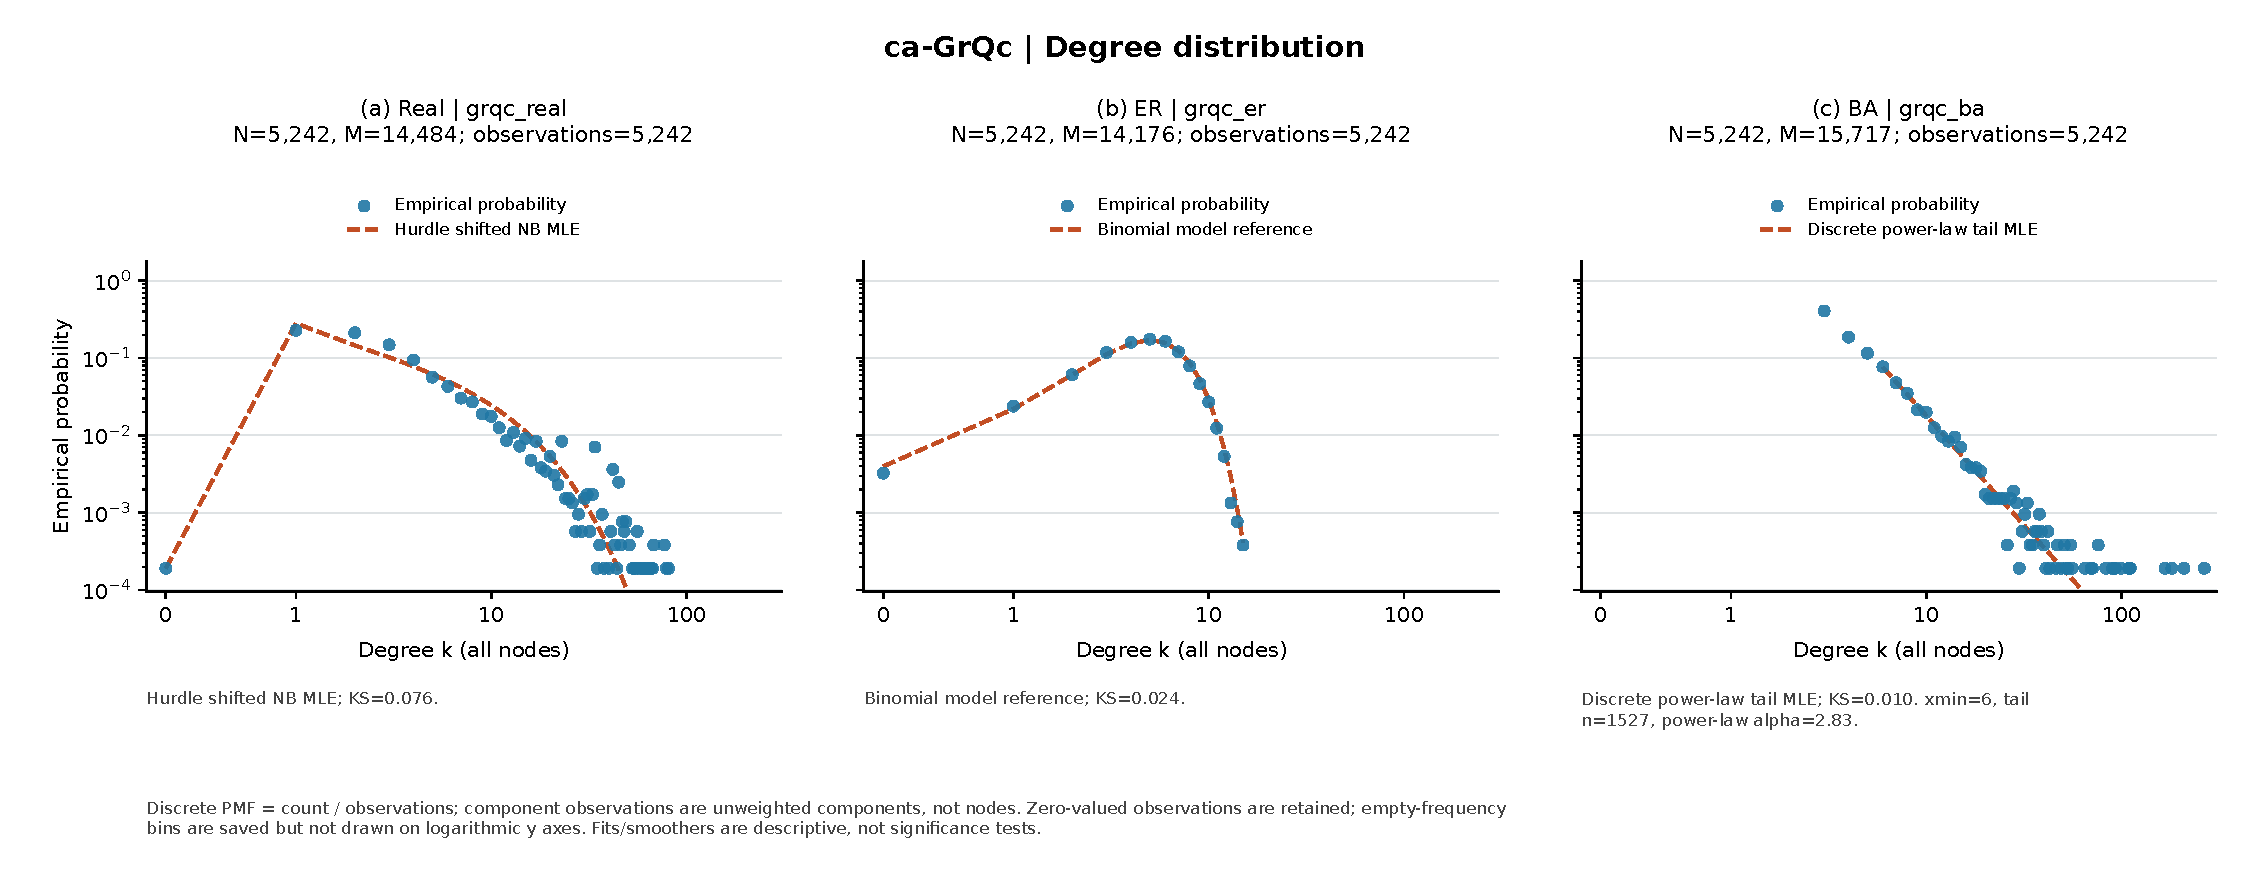
\includegraphics[width=0.96\linewidth]{task3/grqc__degree.pdf}
\caption{\textbf{Degree distributions for ca-GrQc and its ER/BA counterparts.} All nodes are included. Dashed curves show the real-network count fit, ER reference, and BA tail fit, respectively.}
\label{fig:degree-grqc}
\end{figure}
\begin{figure}[!htbp]
\centering\small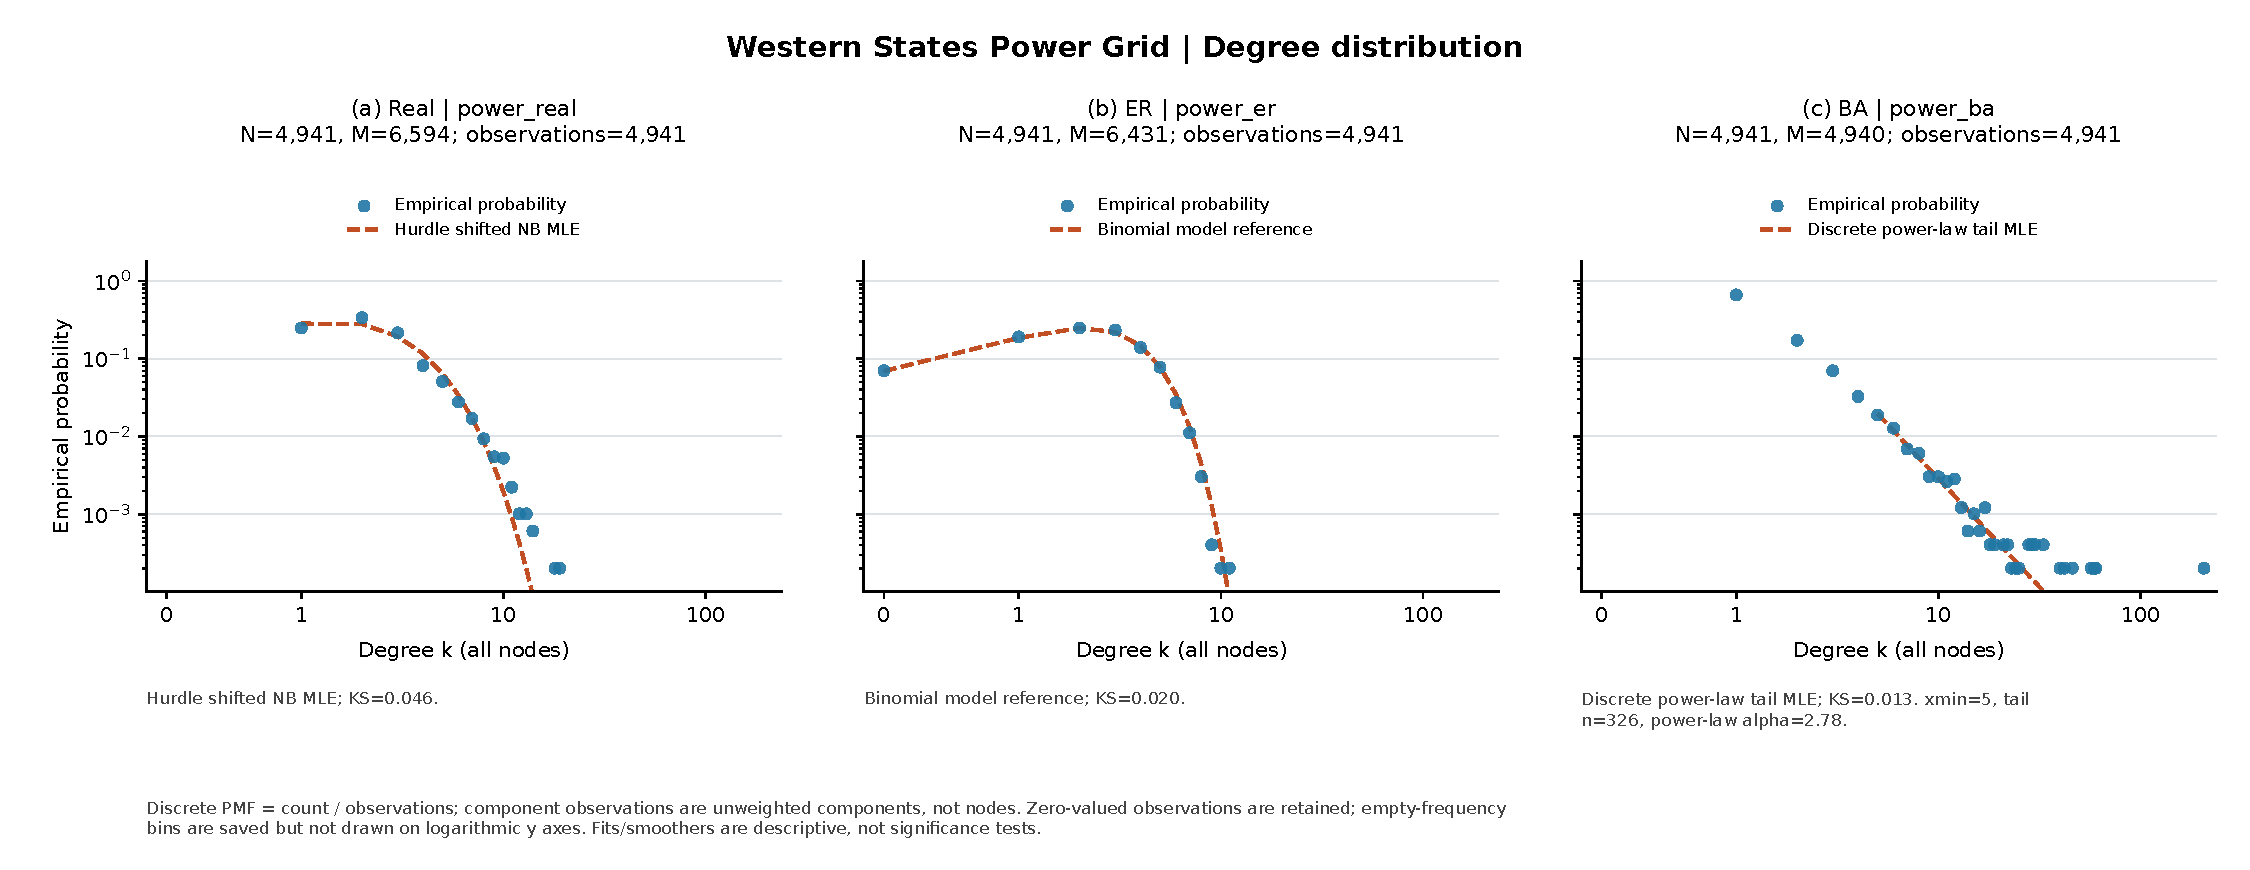
\includegraphics[width=0.96\linewidth]{task3/power__degree.pdf}
\caption{\textbf{Degree distributions for Power Grid and its ER/BA counterparts.} The BA curve describes degrees $k\geq5$ only; the full empirical distribution is retained.}
\label{fig:degree-power}
\end{figure}
\clearpage

\subsection{Longest-Shortest-Path (Eccentricity) Distribution}
Eccentricity is $e(v)=\max_{u\in\mathrm{LCC}}d(v,u)$, measured in hops. Figures~\ref{fig:ecc-grqc} and~\ref{fig:ecc-power} use one observation per LCC node. Curves are bounded discrete-normal fits, except for Power Grid BA, which uses a beta-binomial fit. All curves are restricted to the observed integer support from radius to diameter.

\begin{figure}[!htbp]
\centering\small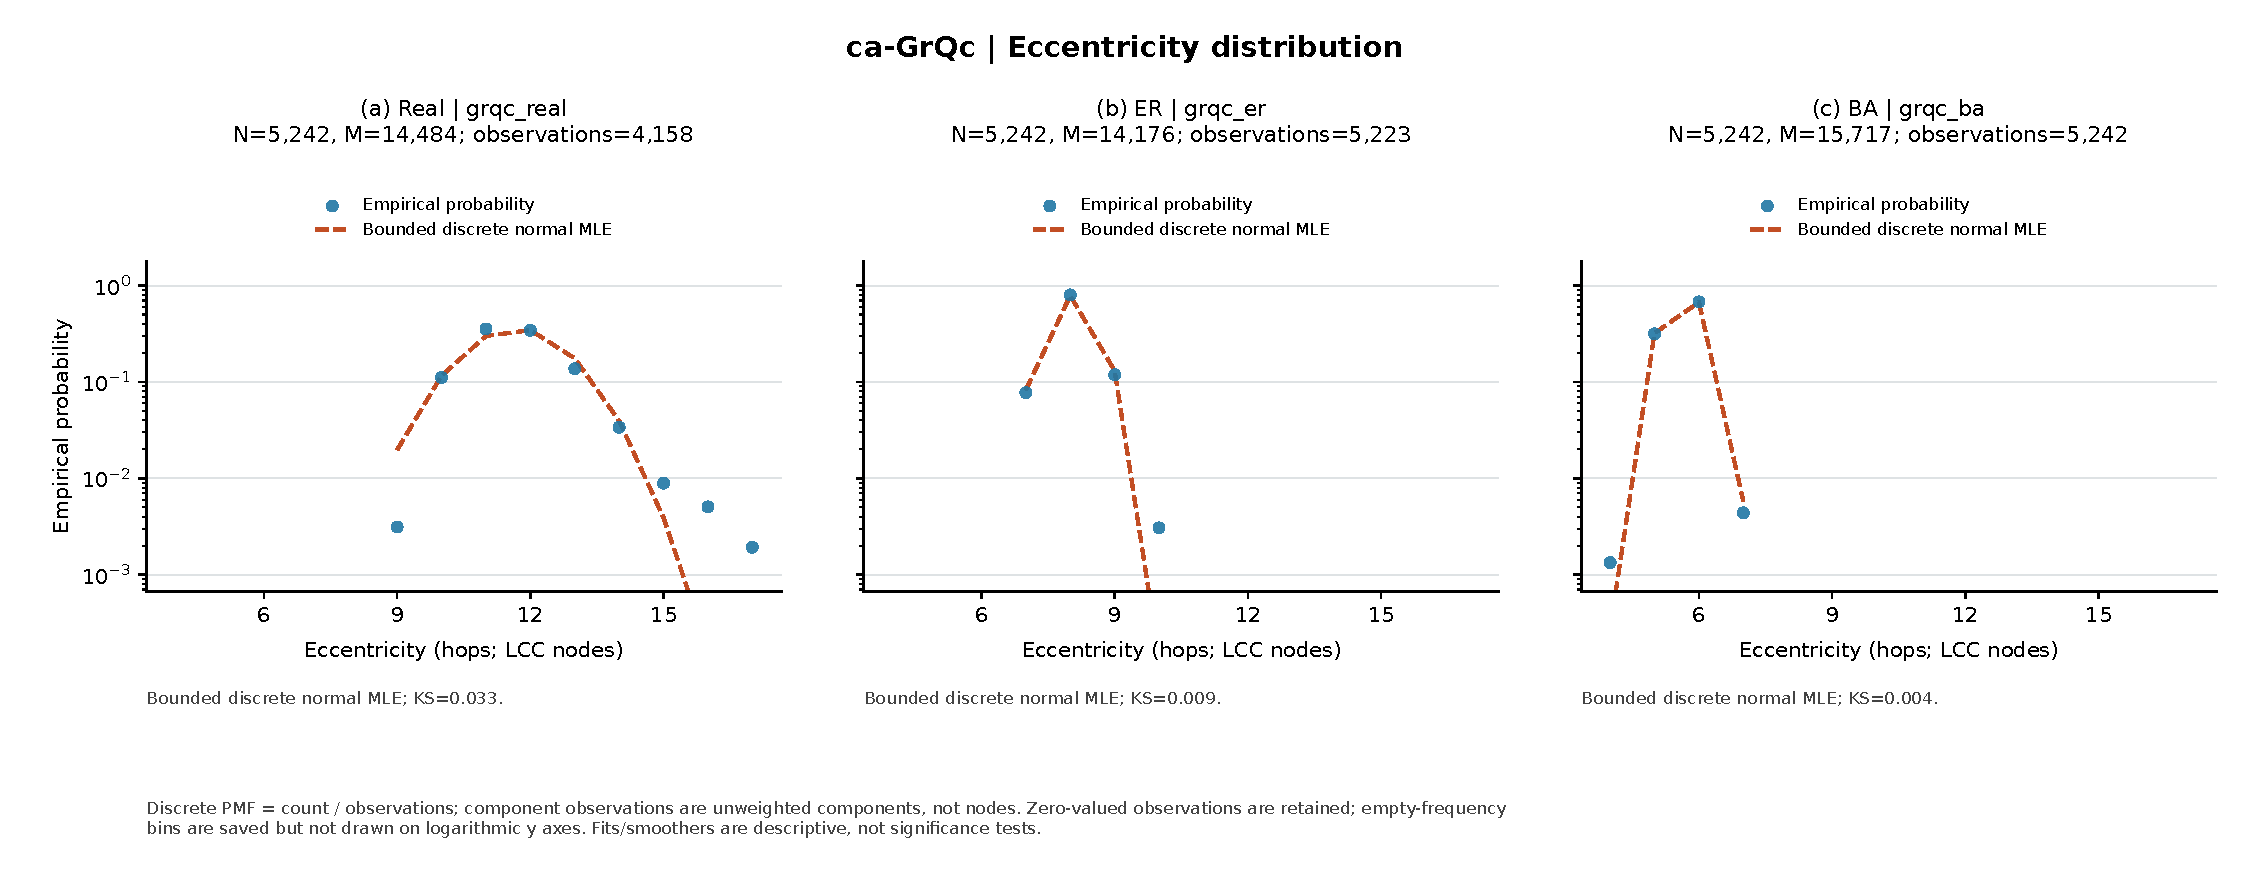
\includegraphics[width=0.96\linewidth]{task3/grqc__eccentricity.pdf}
\caption{\textbf{Eccentricity distributions for ca-GrQc and its ER/BA counterparts.} Each observation is an LCC node. Dashed curves are bounded discrete-normal fits on the observed integer supports.}
\label{fig:ecc-grqc}
\end{figure}
\begin{figure}[!htbp]
\centering\small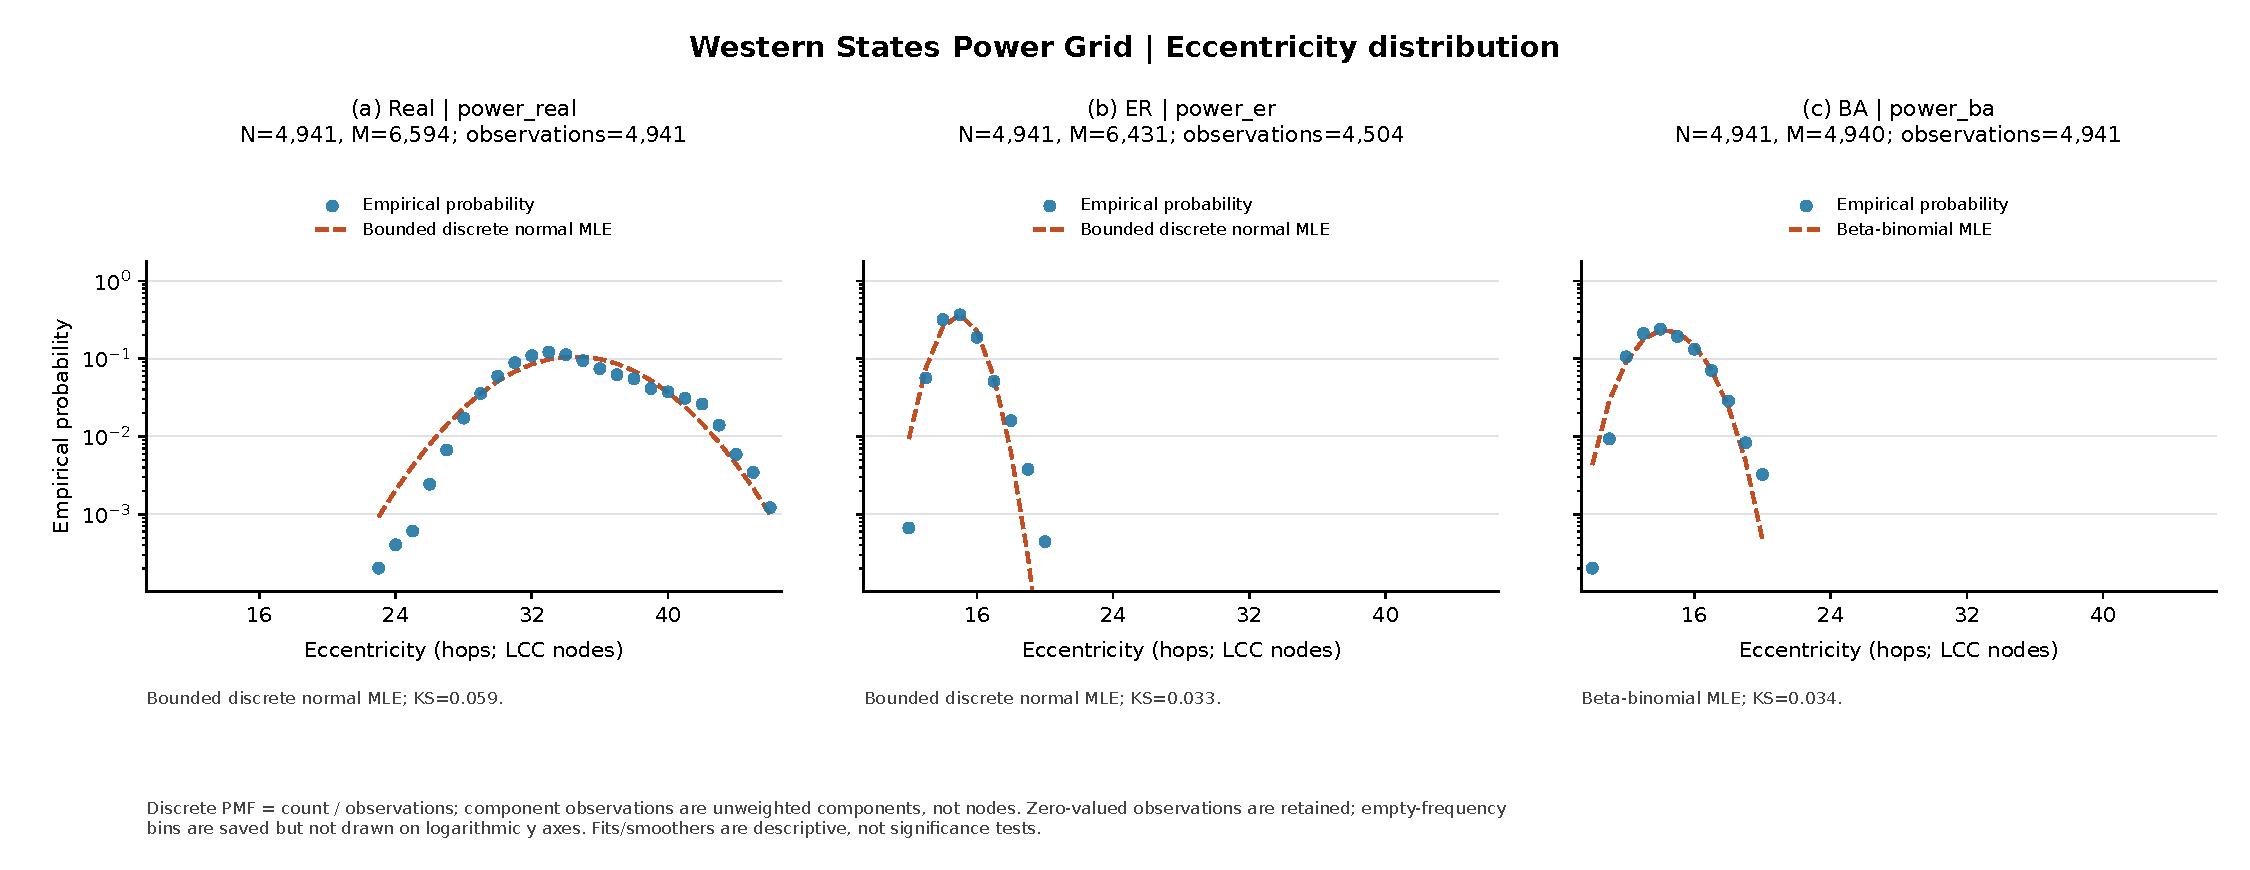
\includegraphics[width=0.96\linewidth]{task3/power__eccentricity.pdf}
\caption{\textbf{Eccentricity distributions for Power Grid and its ER/BA counterparts.} Curves are bounded discrete-normal fits for real/ER and a beta-binomial fit for BA. Distances are in hops.}
\label{fig:ecc-power}
\end{figure}
\clearpage

\subsection{Clustering-Coefficient Distribution}
Figures~\ref{fig:clustering-grqc} and~\ref{fig:clustering-power} include all nodes, assigning zero to degree-zero/one nodes. Four curves use reflected kernel density estimation (KDE), integrated over bins, as descriptive smoothers after Beta fits failed the selected screen. Continuous fits are N/A for Power Grid ER (eight interior observations) and BA (all-zero clustering because $m=1$ produces a tree).

\begin{figure}[!htbp]
\centering\small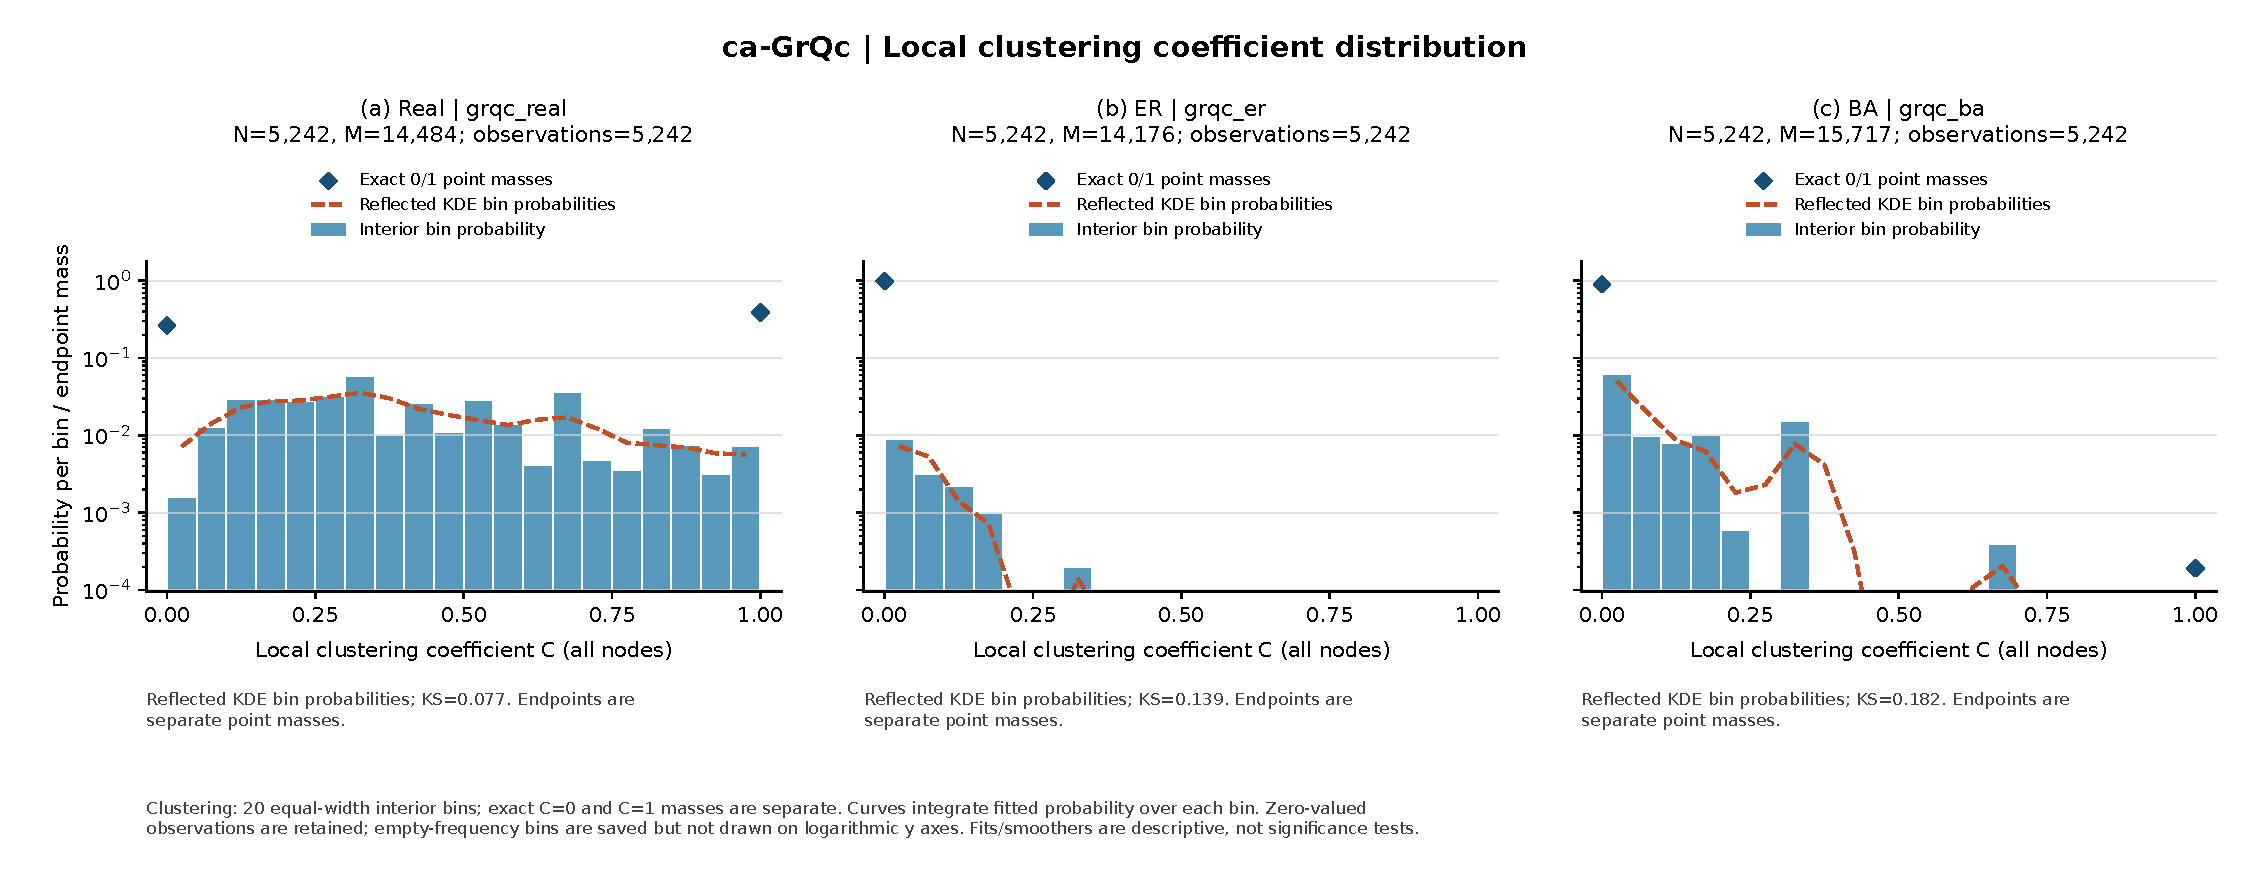
\includegraphics[width=0.96\linewidth]{task3/grqc__clustering.pdf}
\caption{\textbf{Local clustering distributions for ca-GrQc and its ER/BA counterparts.} Bars show interior probabilities, diamonds show endpoint masses, and dashed curves show KDE bin probabilities.}
\label{fig:clustering-grqc}
\end{figure}
\begin{figure}[!htbp]
\centering\small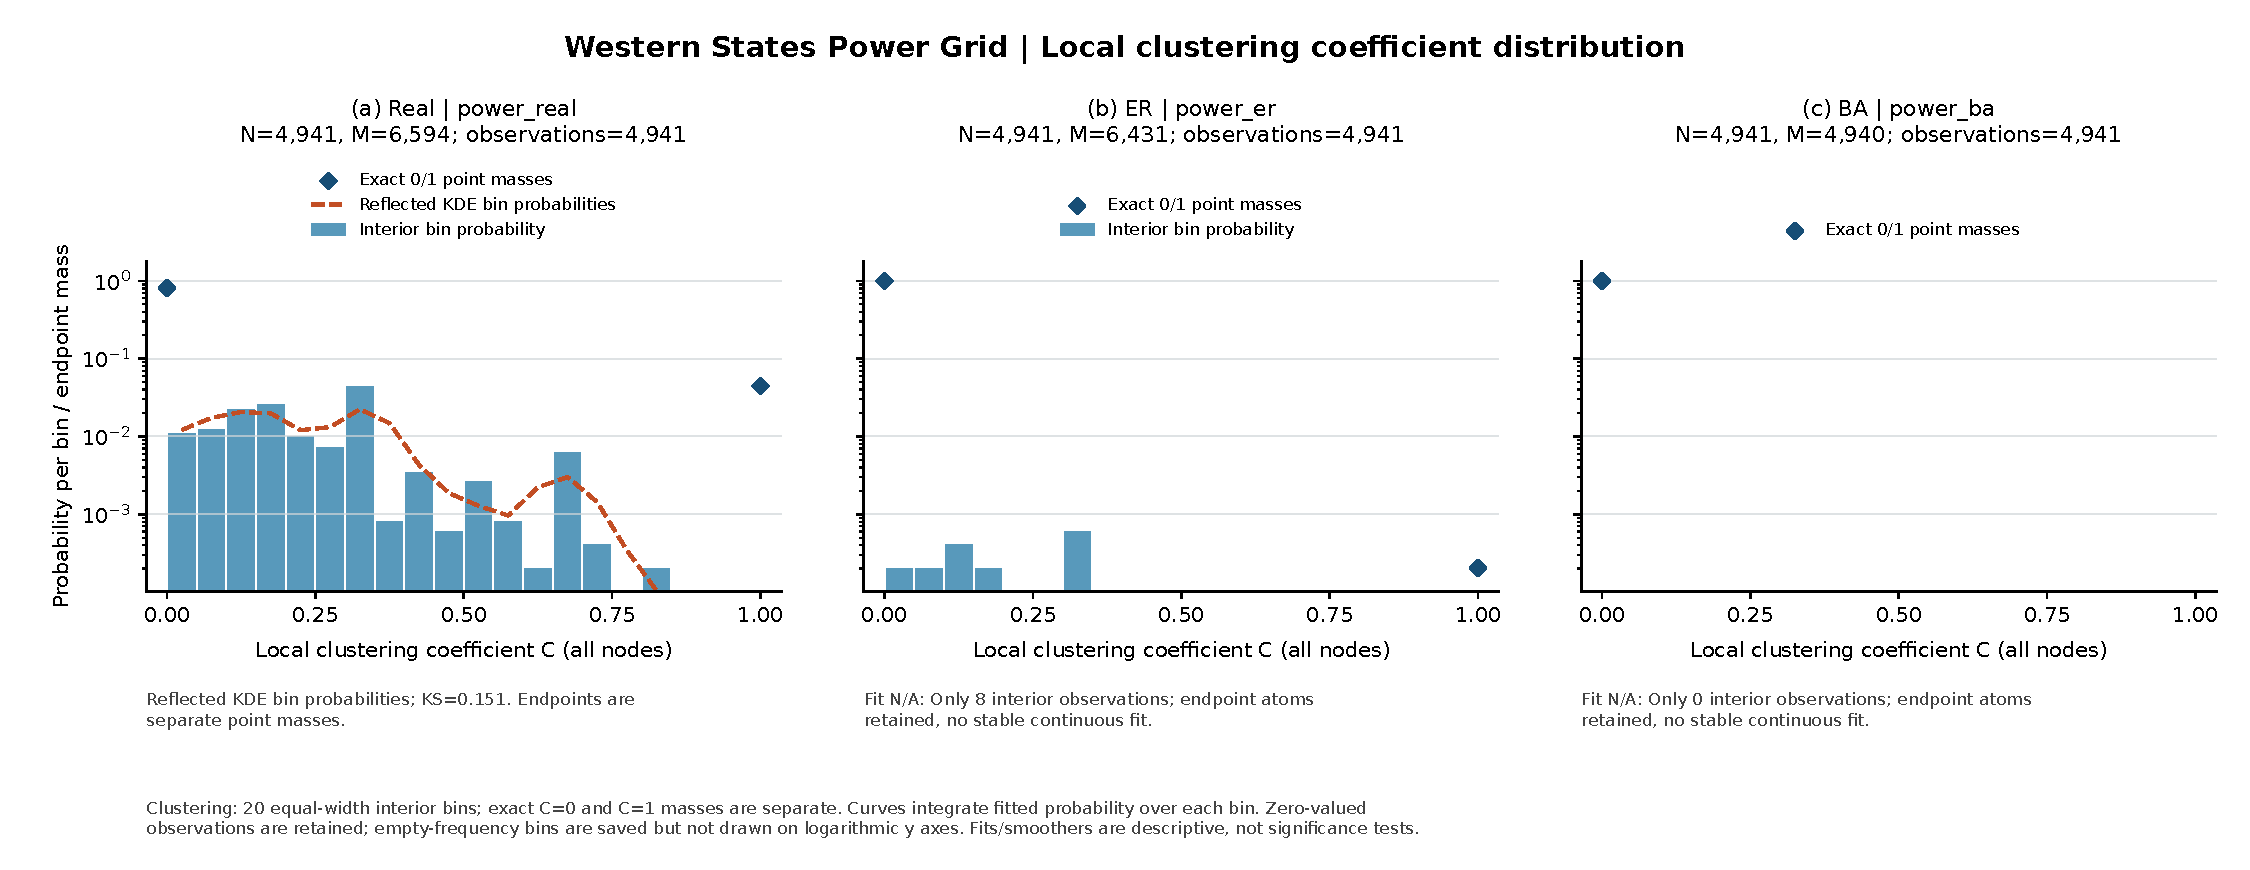
\includegraphics[width=0.96\linewidth]{task3/power__clustering.pdf}
\caption{\textbf{Local clustering distributions for Power Grid and its ER/BA counterparts.} The real-network curve is a KDE smoother. ER/BA fits are N/A; all nodes are included.}
\label{fig:clustering-power}
\end{figure}
\clearpage

\subsection{Connected-Component Size Distribution}
Figures~\ref{fig:components-grqc} and~\ref{fig:components-power} weight components equally. Power Grid ER fits non-LCC sizes with a shifted negative binomial, scaled by their component fraction. Fits are N/A for connected graphs (one observation), real ca-GrQc (failed fit screen), and ca-GrQc ER (18 non-LCC observations). The latter two follow the chosen fitting policy. All moments include the LCC.

\begin{figure}[!htbp]
\centering\small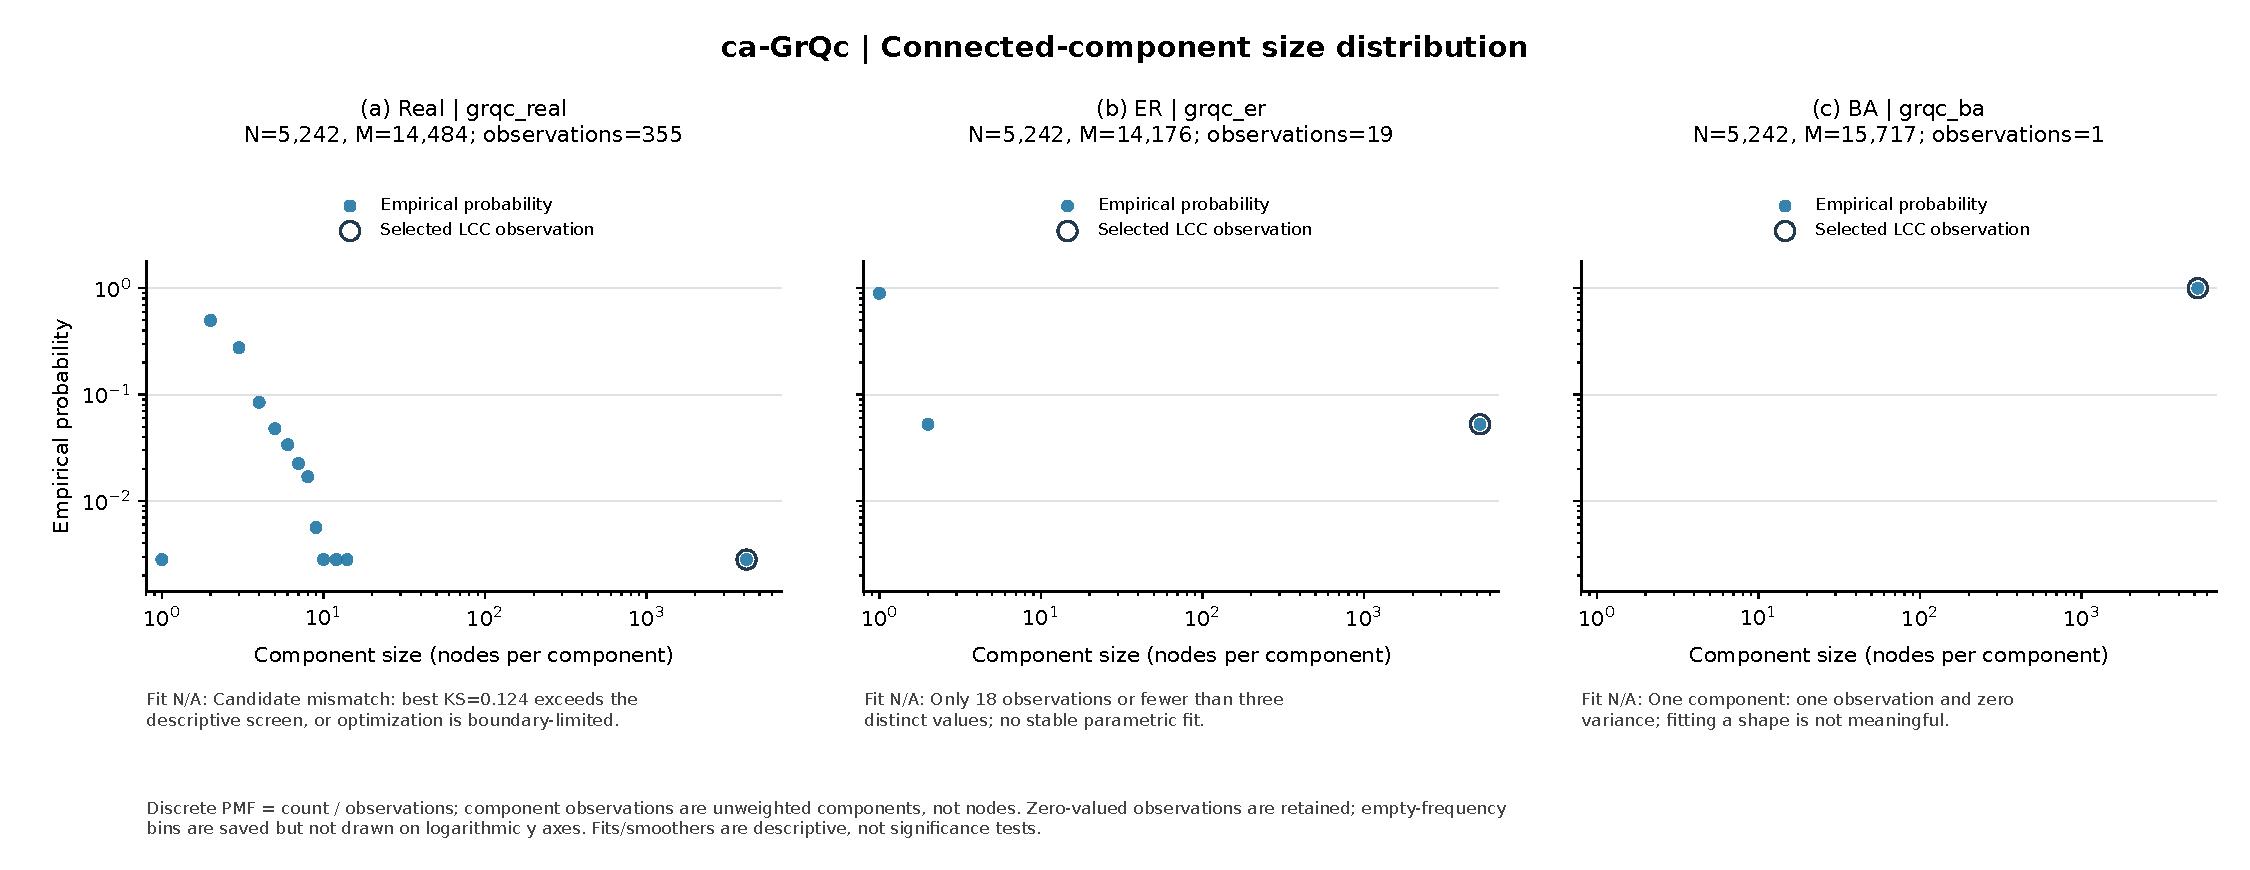
\includegraphics[width=0.96\linewidth]{task3/grqc__component_size.pdf}
\caption{\textbf{Component-size distributions for ca-GrQc and its ER/BA counterparts.} Probabilities are per component, not per node. All components are shown; N/A annotations explain the omitted curves.}
\label{fig:components-grqc}
\end{figure}
\begin{figure}[!htbp]
\centering\small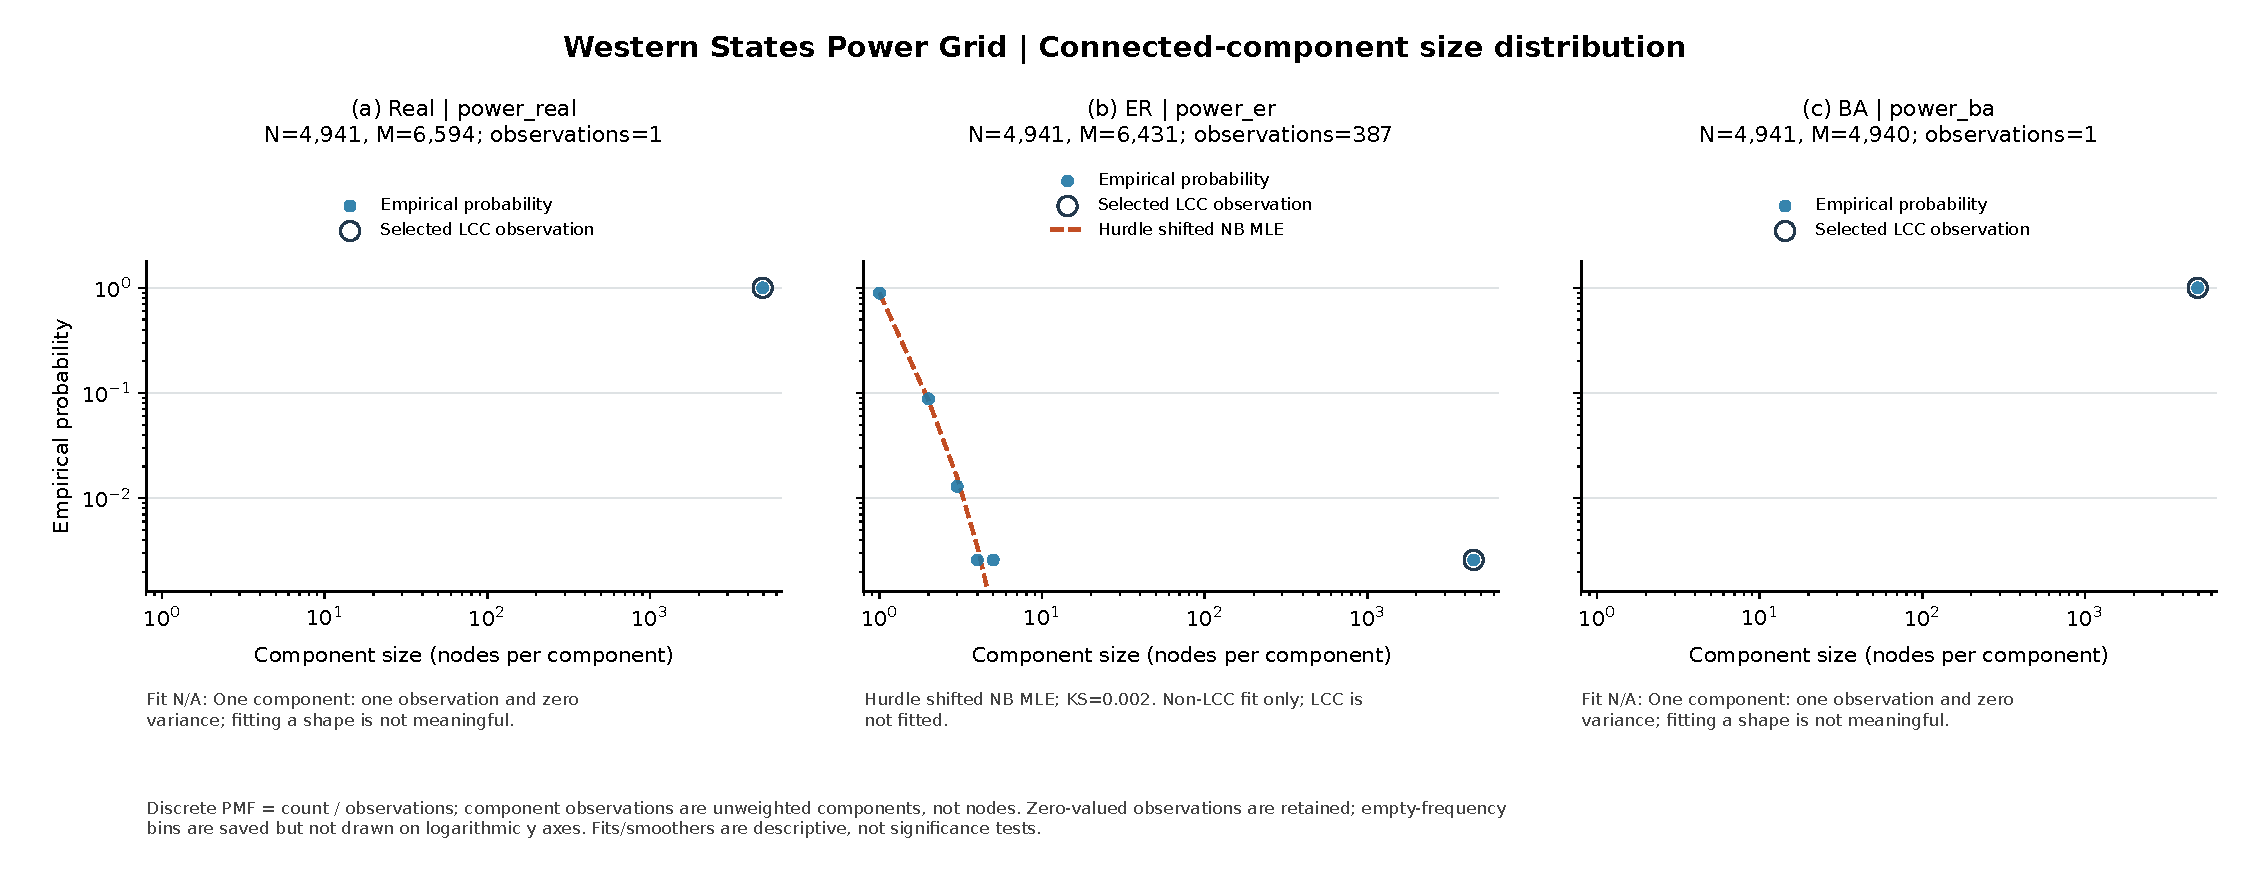
\includegraphics[width=0.96\linewidth]{task3/power__component_size.pdf}
\caption{\textbf{Component-size distributions for Power Grid and its ER/BA counterparts.} The ER curve fits non-LCC components only; the LCC and single-component real/BA graphs remain empirical observations.}
\label{fig:components-power}
\end{figure}
\clearpage
\endgroup
